% MEng project
% CH1 --- background
%
\documentclass[12pt, a4paper, pdflatex, leqno, twoside, openright]{report}

% Define margins
\usepackage[a4paper,inner=40mm,outer=20mm,top=20mm,bottom=25mm,pdftex]{geometry}

\usepackage[T1]{fontenc} % polsih

% Harvard citation
\usepackage[square]{natbib}
\usepackage{cite} % BiTeX

\usepackage{graphicx}
\usepackage{caption}
\usepackage{subcaption}
\usepackage{url}
\usepackage{listings}
\usepackage{minted}
\definecolor{Bkgd}{rgb}{0.98,0.98,0.98}

\usepackage{datetime}
\newdateformat{monthyeardate}{%
  \monthname[\THEMONTH] \THEYEAR}

% New commands
\newcommand{\ts}{\textsuperscript}
\newcommand{\HRule}{\rule{\linewidth}{0.5mm}}

\newenvironment{dedication}
  {\clearpage               % we want a new page
   \thispagestyle{empty}    % no header and footer
   \vspace*{\stretch{1}}    % some space at the top 
   \itshape                 % the text is in italics
   % \raggedleft            % flush to the right margin
   \raggedright             % flush to the right margin
   \par\setlength{\leftskip}{0.3\textwidth}\noindent\ignorespaces
  }
  {\par                     % end the paragraph
   \vspace{\stretch{3}}     % space at bottom is three times that at the top
   \clearpage               % finish off the page
  }

\usepackage{lipsum}

\usepackage{amsmath}
\usepackage{scalerel}
\DeclareMathOperator*{\Bigcdot}{\scalerel*{\cdot}{\bigodot}}

\begin{document}

\begin{titlepage}
  \begin{center}

\includegraphics[width=0.5\textwidth]{gfx/UOB-logo.png}~\\[2.5cm]

\HRule \\[0.4cm]
{\huge \bfseries
  {\Huge Building activity recognition model:}\\[0.1cm]
  learning Prolog rules and extracting features from spatio-temporal data\\[0.4cm]
}
\HRule \\[1.5cm]

    \begin{minipage}{0.4\textwidth}
      \begin{flushleft} \large
\emph{Author:}\\
Kacper B. \textsc{\textbf{Sokol}}
      \end{flushleft}
    \end{minipage}
    \begin{minipage}{0.4\textwidth}
      \begin{flushright} \large
\emph{Supervisor:} \\
Prof.\ Peter \textsc{\textbf{Flach}}
      \end{flushright}
    \end{minipage}

\let\thefootnote\relax\footnote{\hspace*{-1.7em}Level M/7 $|$ COMSM0130---40cp Individual Project}

\vfill % Bottom of the page
{\large \today}
  \end{center}
\end{titlepage}

\newpage
\thispagestyle{empty}
\mbox{}

\newpage
\thispagestyle{empty}
\mbox{}

% Acknowledgement
\begin{center}\textbf{Declaration}\\[1em]\end{center}
This dissertation is submitted to the University of Bristol in accordance with the requirements of the degree of Master of Engineering in the Faculty of Engineering. It has not been submitted for any other degree or diploma of any examining body. Except where specifically acknowledged, it is all the work of the Author.\\[1.5cm]
Kacper B.\ Sokol, \monthyeardate\today

\newpage
\thispagestyle{empty}
\mbox{}

% Abstract
\begin{abstract}
\thispagestyle{empty}
This project researches \texttt{Prolog}'s \emph{Inductive Logic Programming} approach to learn parametrised rules describing \emph{Activities of Daily Life} based on data acquired form smart-houses: premises equipped with vast number of sensors.\\

To this end, highly customisable smart-house data generator is constructed and capabilities of \texttt{Aleph} inductive logic programming framework are assessed on various spatio-temporal datasets. Subsequently, \emph{Activity Recognition Model} is constructed based on data collected from simulations and Washington State University CASAS smart-house installations. Both single and multiple occupiers models are considered.\\

To achieve aforementioned goals, signal issues such as noise and incompleteness among others are addressed. Furthermore, method for raw data transformation into logical facts is proposed and evaluated. Difficulties such as real-valued sensor output and time representation in first-order logic are described.\\

The second objective of this work is to examine structure of used spatio-temporal data with a view to discover and form new features. To this end, dependencies between sensors are identified and assessed in order to construct more informative features. Hence, by extending dataset with new features performance of any classification algorithm can be significantly boosted.\\

Finally, \emph{Narrative Analytics} is proposed: an extension of Activity Recognition Model transforming generated rules into \emph{natural language}. Introduced data visualisation technique produces plain English description of monitored premise, hence, house situation can be recognised without time consuming data interpretation.\\

The main utilisation of proposed here techniques is house monitoring for healthcare applications. SPHERE Project hosted at the University of Bristol addresses increasing healthcare costs and decreasing quality of life by designing tools and techniques allowing patients to live at home regardless of their medical conditions.\\
Described in this paper activity recognition approach aims at improving classification results and presenting smart-house data in a more transparent way. To the best of my knowledge, presented here methods are first of its kind and has not been yet described in any publication.

\begin{center}
Keywords: \textbf{Inductive, Logic, Programming, Prolog, Activity, Recognition, Data, Generation, SPHERE}

% \let\thefootnote\relax\footnote{\noindent This publication including source code is available as \texttt{GIT} repository at: \url{https://github.com/So-Cool/cognition}.}
\end{center}
\end{abstract}



\newpage
\thispagestyle{empty}
\mbox{}
\begin{dedication}
``\ldots~On each landing, opposite the lift-shaft, the poster with the enormous face gazed from the wall. It was one of those pictures, which are so contrived that the eyes follow you about when you move. BIG BROTHER IS WATCHING YOU, the caption beneath it ran.~\ldots''\\[1cm]

``\ldots~The telescreen received and transmitted simultaneously. Any sound that Winston made, above the level of a very low whisper, would be picked up by it, moreover, so long as he remained within the field of vision which the metal plaque commanded, he could be seen as well as heard. There was of course no way of knowing whether you were being watched at any given moment. How often, or on what system, the Thought Police plugged in on any individual wire was guesswork. It was even conceivable that they watched everybody all the time. But at any rate they could plug in your wire whenever they wanted to. You had to live did live, from habit that became instinct in the assumption that every sound you made was overheard, and, except in darkness, every movement scrutinized.~\ldots''\\[2cm]

Nineteen Eighty-Four, George Orwell
\end{dedication}


\newpage
\thispagestyle{empty}
\mbox{}

\newpage
\cleardoublepage
\pagenumbering{gobble}
\tableofcontents
\cleardoublepage
\pagenumbering{arabic}

% \newpage
% \thispagestyle{empty}
% \mbox{}

%===============================================================================
%===============================================================================
%===============================================================================
%===============================================================================
%===============================================================================
\chapter{Introduction\label{ch:introduction}} %Background
\setcounter{page}{1}
% -------- plain English -> explain to someone
% Start with motivation - what is the problem and why it's interesting
% SPHERE somewhere here
% and application - what to do with it
% give solution
% then technique - why technique is best for solution - and more technical details
% --------
% What the project will produce -> contribution
% level of technical challenge
% how the output will be assessed - evaluation
% --------

  \section{The activity recognition}
    \subsection{Outline} %Problem outline
The main aim of the project is to build \emph{activity recognition model} for \emph{smart house} monitoring purposes.\\
By the latter I understand a premise that is fitted with variety of sensors like: motion, door, appliances, water, item, etc.; as well as more sophisticated monitoring devices like cameras, and depth cameras. The first kind of sensors generate raw output usually of a form \texttt{sensorID on}/\texttt{sensorID off}, while the latter type outputs complex signal that needs to be pre-processed to be used as an input of classifiers. Due to aforementioned sensor characteristics my work is mainly focus on the first type of sensors.\\
Therefore in presented above scenario, activity recognition model is a set of techniques that applied to real time signals generated by a house produce a prediction of currently held activity like \emph{cooking} or \emph{sleeping} assigned to one of the premise \emph{residents}. The best solution to sketched above problem is one that works in \emph{signal streaming environment} therefore producing real-time activity predictions with high recognition rate.

    \subsection{Motivation\label{sec:applications}} %Problem motivation/Applications
% Why interesting -> it generalises to any spatio-temporal data therefore can be used
Proposed here activity recognition model is a special case of \emph{predictive model} for \emph{spatio-temporal} data. In general such techniques predict quantity of interest based on input data that encode both location and time of the event of interest.\\
% Why is it needed -> spatio-temporal data is everywhere,
This generalisation have wide variety of real-life applications therefore addressing problems defined as ``hard'' in the activity recognition literature would make valuable contribution to the field. 
First and foremost area of application is healthcare.
% Population ageing - society geting older,  SPHERE project

      \subsubsection{Healthcare: The SPHERE Project}
Allowing elderly people and clinical patients to live at home regardless of health conditions they suffer greatly benefits such individuals. Dwelling in cosy environment causes less stress and individuals being located at home means no need for specialistic day care centres and less crowded hospitals.\\
Therefore, being able to monitor behaviour of people in their own houses and effectively describe their activities result in better patient care possibilities. Such methods allow quick response to any kind of incidents without disturbing monitored people when it is unnecessary.

\begin{figure}
  \centering
  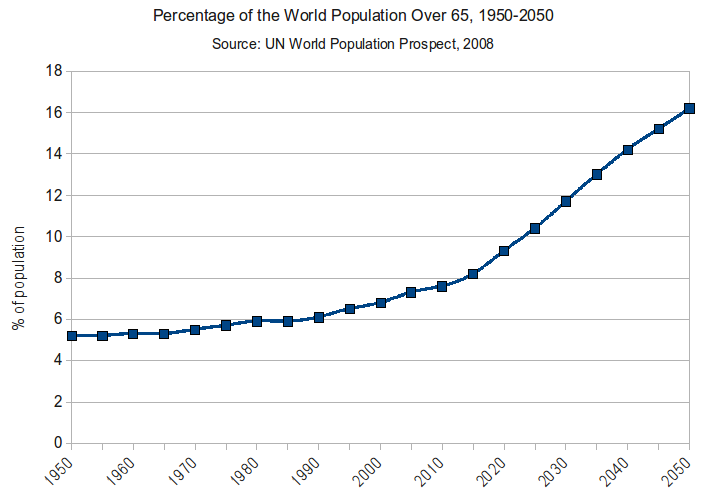
\includegraphics[scale=.5]{./gfx/populationOver65}
  \caption{Percentage of world population over 65, 1950--2050; \citep{populationAgeing}.\label{fig:agingPopulatiom}}
\end{figure}

% The Challenge
The problems of ageing population (see \emph{Figure~\ref{fig:agingPopulatiom}}), global population health issues, increasing healthcare costs, and decreasing quality of life are addressed by the \emph{SPHERE Project} hosted at the University of Bristol \citep{sphere}. This collaboration of clinicians, engineers, designers, social care professionals and various members of the public develops helpful technologies addressing real healthcare problems in a cost effective way.\\
The project focuses on developing real-world technologies which are acceptable in people's homes i.e.\ do not hindering everyday-life. SPHERE works on both hardware and software smart house solutions: sensors and wearable devices as well as algorithms for healthcare applications. The first, are fitted in the place of interest to monitor it and generate various kind of signals, while the latter, use acquired information to identify medical or well-being issues: predict falls, detect strokes, analyse eating behaviour, and detect periods of depression or anxiety.\\
This project extends algorithmic part of undertaken by SPHERE research by proposing novel data analysis framework.

      \subsubsection{Smart City}
Despite huge popularity in healthcare, spatio-temporal data feeds can also be found in variety of monitoring applications. One of them described by \citet{filipponi2010smart} is smart-city management. Automatic analysis---quick and robust---of traffic information, accident reports, etc.\ is of invaluable help in case of emergency.\\
Among many possible applications, produced analysis can result in timely police intervention or well planned route for emergency services, therefore, help in evacuation, crowd management, terrorist attack prevention and airport security control.

      \subsubsection{Complex Systems}
Spatio-temporal data are also produced in large quantities by many of complex systems monitoring and control devices, e.g.: scientific facilities, buildings, data centres~\citep{moore2005data} and power plants~\citep{amin2005toward}. 
Tasks impossible to handle by humans either due to large data volume throughput or demand for low response time are vast area of application for spatio-temporal data analysis. Such tools facilitate well suited for needs system management and risk detection. Power distribution and balancing, nuclear reactor control, data centre heat management are such tasks to name a few.

      \subsubsection{Wildlife}
Monitoring animals behaviour in their natural habitat is an important source of information for many researchers~\citep{Szewczyk:2004:HMS:990680.990704}. Nevertheless, this task is very often impractical either due to adverse climate or difficult access to monitored place. Moreover, scientists in many cases want to avoid disturbing animals' life-cycle and habitats. Difficult access to such sites can be easily overcome with wide range of available sensors and analytic tools, which share common ground with activity recognition model.


  \section{Contribution}
    \subsection{Existing work}
Over the last few years, building machine learning models for \emph{Activity of Daily Living} (ADL) has become an interest of many researchers. Its wide area of applications and increasing complexity appearing with every new discovery attracts now and then machine learning community with new and innovating ideas.\\

    \subsubsection{Techniques}
Up to date, extensive work on houses occupied with both \emph{single}~\citep{cook2009assessing,fatima2013unified} and \emph{multiple}~\citep{hsu2010strategies,singla2010recognizing,crandall2009coping} residents has been done, nevertheless, vast majority focused on state-of-the-art learning algorithm such as:
\begin{itemize}
\item transfer learning---\citet{cook2013transfer},
\item conditional random field---\citet{hsu2010strategies,van2010activity},
\item support vector machines with various kernels---\citet{fatima2013unified},
\item hidden Markov model---\citet{rashidi2011discovering},
\item na\"{\i}ve Bayes---\citet{cook2013activity},
\item artificial neural networks---\citet{fatima2013unified,fatima2013analysis}.
\end{itemize}

All of these models are fuelled by variety of features extracted from raw signals by transformation and time manipulation. Majority of undertaken work in this field uses motion sensors as main source for feature construction with little to none attention to item sensors.\\

Unfortunately, scientific environment focuses on mainstream models and forget about possibly simpler and more suitable but less popular techniques. Observing this gap in spatio-temporal data analysis opens vast new area of research of building activity recognition models with less popular machine learning techniques which is addressed in this paper.

      \subsubsection{Datasets}
Training and testing any activity recognition model requires a dataset of recorded human activities. Such data can be only obtained by designing and building a test-bed house fitted with variety of sensors followed by numerous ``plays'' of scripted activities. As majority of researchers cannot invest time or money to construct a smart house they use publicly available datasets generated by one of research facilities. The most popular choice~\citep{fatima2013unified,fatima2013analysis,nazerfard2010conditional,cook2009assessing} among researchers are datasets published by \citet{cook2009assessing} working at \emph{Center for Advanced Studies in Adaptive Systems}, Washington State University; also known as \emph{CASAS datasets}.\\
Their popularity is based on large amount of variety of recorded activities, with both single and multiple occupiers, available publicly free of charge. Furthermore, they are fairly well formatted and documented nevertheless, they sometimes show inconsistency with labelling structure.

      \subsubsection{Issues}
Tasks such as activity recognition aim at predicting nearly infinite amount of human activities which can be performed in variety of manners. This enormous complexity of the task causes numerous problems ranging from activity prediction, to assigning one of multiple occupiers to performed task. Such ``multi layered'' predictions yield many possibilities for assessing performance e.g.\ correct activity, wrong agent prediction; correct activity, correct agent prediction; etc..\\

The literature identifies building model for some of the activities as relatively difficult. Many of them involve complex, time consuming tasks with multiple residents crossing each others paths. Some of them are addressed in latter parts of this work.\\

Finally, due to specific to dataset output formatting and sensor name-space learnt models are not universal.

      \subsubsection{Outcomes}
Outcomes of activity modelling tasks reported in the literature are unfortunately poor reference for assessing model performance. Use of different datasets and fitness measures depending on study make result comparison impractical.\\
For instance,~\citet{fatima2013analysis} report \emph{accuracy} ranging from $\sim0.2$ to $\sim1.0$ depending on model, dataset and predicted activity.


    \subsection{Project contribution}
Broad activity recognition literature and variety of tested therein models clearly indicate that no single classifier can handle diversity of activity structures embedded in the data. Each model has its pros and cons therefore perfect solution should use all of the models offering features not covered by the others---the concept known as \emph{ensemble learning}.\\

As none of published so far piece of literature discusses application of \emph{first-order formulas} i.e.\ parametrised logical rules, as building blocks of activity recognition model this work comprehensibly covers this problem to expand collection of used techniques. Therefore, the main aim of the project is to apply \emph{Inductive Logic Programming} (ILP) techniques to spatio-temporal data acquired from ``smart'' installations---houses in particular---in order to build \emph{Activity Recognition Model} and extract new, more informative features from raw signals.\\

To address the first problem capabilities of ILP system and model description via set of first-order logical rules are investigated. Both cases: houses with single and multiple occupiers are examined.\\
The latter task involves critical analysis of designed for model learning signal features and assessing their quality. Such novel signal characteristics can be used in any other activity recognition model to boost its performance.\\

Designing a new model and signal features can become difficult task when exact structure of used dataset is unknown. Therefore, systematic way of \emph{generating smart-house data} within user controlled environment is desirable. As part of this project highly customisable data generator is proposed. Such tool facilitates generating datasets representing activities of arbitrary complexity therefore produced data can be used to build and test activity recognition models in (in)deterministic world simulation. Moreover, produced by the generator datasets are invaluable help to systematically compare and contrasting all the learning methods.\\

Finally, the project aims at proposing \emph{unified activity-recognition model evaluation measures}. A systematic way of assessing performance of classifier in activity recognition tasks is beneficial for comparing and contrasting multiple solutions. With such techniques unambiguous assessment of multiple methods for particular activity is possible yielding obvious identification of best solution.

\section{Techniques}
To achieve set above goals performance of proposed technique is evaluate on both \emph{CASAS datasets} and \emph{CASAS-inspired synthetic} datasets produced by the generator. Both datasets are translated from log-like format into \emph{knowledge representation} i.e.\ sensor readings are expressed as logical facts. The evaluation is made by means of \emph{cross-validation}. CASAS datasets are split into activities per person to produce folds so that each fold contains number of activities performed by single person. On the other hand, when evaluating synthetic data each fold is generated independently with common activity structure and small variation of order of used items and detours from originally planned motion trajectory.\\

% why I think it's best for the problem -> more details
The core of proposed technique is \texttt{ALEPH}---Inductive Logic Programming system producing \texttt{Prolog} clauses as the model of data. This approach to learning activity recognition model was chosen as it lacks needed attention in the subject literature.\\

Proposed here rule based classifier greatly differs from currently used methods. Instead of employing \emph{propositional logic} it uses more powerful first-order logic, to express data and activity structure believes. More advanced ``grammar'' implies more possibilities to express complex relations between sensor events. This extra power can be harnessed to compose new data features which can be used in training other models and potentially improve their performance.\\

Furthermore, expressing the activity model in \texttt{Prolog} programming language brings to power all its advantages. Easy \emph{search space traversal} and built-in \emph{negation as failure} are invaluable tools in feature construction. Finally, learnt activity recognition model can be easily transformed to a \emph{generative model} for data hence, serve as an activity example generator.\\
\texttt{Prolog} is also well known for its \emph{natural language processing} capabilities. Rule based model can be therefore used to produce \emph{Data Narrative}---a plain English interpretation of the data which supersedes any other visualisation technique targeted at general public.\\

Another advantage of ILP learning is use of \emph{background knowledge}. It encodes \emph{clauses} needed to build the target model but can also contain any information or rules that might be beneficial for raw data interaction.\\
In smart-house model such component is of invaluable help as it can contain all the house and activity details that are absent in raw data. Room layout, sensor placement, activity structure are just some of them.\\
Moreover, background knowledge acts as a \emph{proxy} between raw data and model, making the latter universal. It means that in majority of cases model learnt for one dataset can be applied to any other by using data-specific background knowledge.\\

Very often monitored activities exhibit hierarchy and structure. Rule based model allow to easily adjust the \emph{resolution of prediction} therefore, activities can be described with different level of depth. Considering activity of eating, the model can simply predict the activity: \emph{eating}; it can also suggest meal type (breakfast, lunch, brunch, etc.) based on time of day; or even food type (pasta, pizza, etc.) based on used ingredients.\\

Rule based model has one more distinctive feature not exhibited by many other machine learning models: it is \emph{human readable}. Such models are easy to inspect and tune simply by eye-balling. Rules can be evaluated whether they make sense, obscure information can be discover and gained knowledge used to design new more suitable features in iterative manner. Rule manipulation is also feasible therefore, they can be simplified (by removing predicate), extended (by appending predicate), or combined (by enclosing them in meta-rule).\\

\section{Deliverables}
% Deliverables / contribution -> what the project will result in
The project delivers highly customizable smart-house data generator written in \texttt{Python}. It is publicly available as a \texttt{GitHub} repository\footnote{\noindent\url{https://github.com/So-Cool/SHgen}} to help researchers with training and testing models.\\
The smart-house simulator is highly customisable: room layout, motion and item sensor placement, and number of occupiers can be specified. The user specifies \emph{action script} which is then ``played'' by house occupiers what in turn produces sensor activations which are recorded in CASAS-like format.\\
As all the actions are ``directed'' precise \emph{ground truth} information is available. Presence of \emph{activity labels} in the data and precise control over the sensor interactions is of invaluable help in experiments of this kind. Finally, the data generator is proved to produces real-like data therefore it is sound for use in model creation and evaluation.\\
The generator repository contains detailed design and usage description to be easy to set-up and use for anybody. The choice of programming language was made based on its popularity making contribution, maintenance and development easy for whole community.\\

Moreover, the project studies in great detail application of ILP to various smart-house settings. Signal output as knowledge representation is proposed. Activity recognition problems defined in literature as ``hard'' for both single and multiple residents are attempted and quality of results is discussed. The capabilities, limitations and advantages of ILP in described scenario is thoroughly investigated and illustrated with examples. The role of background knowledge encoding additional signal characteristics is examined. Used signal features are described and their role in model construction is critically evaluated. Finally, result evaluation techniques are proposed and used to score achieved results.

\section{Challenges}
Issues in all layers: data, ILP and result evaluation arise. To overcome them, multiple solutions are presented and tested to select the best possible one for smart-house data analysis.\\

% prediction continuity issues, and readings in time continuity issues
Very often the data collected from smart-houses are corrupted or obscure due to incompleteness and sensor noise. This phenomenon leads to confusing gaps between ``observed'' actions causing model learning difficulties and intermittent prediction space. With help of inductive learning such implicit information---describing intermediate steps between actions---can be inferred to overcome rule creation difficulty and produce logically consistent scenario.\\
Moreover output of smart-house installations is an unlabelled dataset. Filling the missing activity description is manual labour hence it is time consuming and prone to errors. Lack of reliable ground truth information very often causes model learning difficulties.\\

First-order logic data representation has many advantages but it struggles with unbounded variables like real numbers. This drawback imposes limitations on time and real-valued sensor output representation which is crucial for spatio-temporal data. Discovering possible representations and evaluating their usefulness is of great importance.\\

Learning a data model with ILP is a complex process with number of intermediate steps. First, the learning environment of \texttt{Aleph} ILP system has to be configured to build activity recognition model. For this purpose variety of activity rule structures has to be discovered. Then, datasets and activity scripts need to be analysed to find any relevant structures to extract and format them as signal features. To this end, mechanism in form of \texttt{Prolog} rules has to be built.\\
Background knowledge---the main component of \texttt{Aleph}---is a powerful tool. To make the best use of it, its capabilities and limitations must be discovered. Deciding on useful for feature construction information not contained in the original dataset like room and sensor layout is necessary.\\

Adjusting the resolution (level of detail) of achieved prediction is also a significant task. Therefore, right balance in prediction detail and accuracy trade-off has to be found.\\
Handling data of house occupied by multiple residents introduces difficulty of distinguishing them. Well known problem of agents sharing common space or crossing each other paths has to be resolved.\\

Finally, designing the most suitable an universal evaluation technique is crucial for results comparison. The main difficulty of this task are multiple classification error possibilities. The significance of each of them has to be considered to build performance metric that express real-life usefulness of proposed methodology.

\section{Result evaluation}
For the proposed generator to be publicly accepted in the community dealing with smart-house activity recognition the proof of producing real-like data is necessary. Presented here proof is based on treating output of the generator with model learnt on real data and vice versa. This technique aims at assessing similarity between synthetic and real data.\\

% OUtput asses ->
To prove importance of presented here activity recognition work systematic and versatile evaluation technique is necessary. Firstly, similar technique to generator evaluation is used: applying ``synthetic'' model to genuine data and vice versa. Moreover, different than rule based models are used on both type of data to compare their performance against proposed here technique.\\
Evaluation measures such as accuracy per activity, overall accuracy, accuracy per person per activity are used. Furthermore, for single occupier cases the raw signals are translated into \texttt{ARFF} format and different machine learning models from \texttt{Weka} package are applied to it.\\
Finally, all evaluation is based on \emph{cross validation} to make it more robust. The genuine data is split per person so that each fold contains 5 different activities. The synthetic data is generated with random bits based on script corresponding to the genuine data.


%===============================================================================
%===============================================================================
%===============================================================================
%===============================================================================
%===============================================================================
\chapter{Spatio-temporal data\label{ch:stData}}
Spatio-temporal datasets are made of entries encoding event and their occurrence times. Such data are generated by monitoring systems, logging utilities and all kind of smart-instillations like houses and cities. Majority of such datasets are streamed therefore it is implicitly assumed that learning algorithm at any point can look into the past but never see future.\\
This assumption can be utilised in learning algorithms by allowing current prediction to be based on past predictions. Such practice is widely used to boost classifier performance, nevertheless, it bears danger of skewing future predictions by propagating early made error.

  \section{The smart-house data}
My work focuses on smart-house outputs, which is the most popular case of spatio-temporal data. Each entry in such dataset is generated by change of sensor state and is characterised with \emph{time stamp}, \emph{sensor ID} and new \emph{sensor state}.\\
Smart-house data owe their popularity mainly due to importance of activity recognition models (see \emph{Section~\ref{sec:applications}}). Moreover, such datasets can be arbitrary complex as there exist infinite amount of activities that they can represent. Therefore, techniques designed for smart-house data can be generalised for other spatio-temporal cases which usually exhibit less complexity.

    \subsection{CASAS dataset}
Washington State University's CASAS project~\citep{cook2009assessing} is main source of real smart-house datasets used in this study. These datasets are very popular in activity recognition literature due to their large quantity, recorded in variety of testbeds with diverse sensor types: electricity, motion, door, item and appliance (fixed-phone, water, hob). Furthermore, they contain vast amount of activities of different complexity performed by single and multiple occupiers.\\
The datasets structure is transparent, with list of sensor readings, one entry per line of the form:
$$
\text{\texttt{Date}~~\texttt{Time}~~\texttt{SensorID}~~\texttt{SensorState}~~(\texttt{PersonID\_ActivityID}~~\texttt{ActivityState}).}
$$
First four columns are compulsory. 5\ts{th} and 6\ts{th} sparse column is ground truth information and denote blocks of activities, which in multiple resident case are tagged with resident identifier. \texttt{ActivityID} is a name of activity like \emph{cooking}; \texttt{PersonID} is a resident identifier like \emph{residentA}; and \texttt{ActivityStatus} can be either \emph{begin} or \emph{end} where sensor activations placed between these commands contribute to defined activity.\\
Snippets of CASAS dataset are shown in \emph{Listing~\ref{lst:CASASoneR}} for single resident and in \emph{Listing~\ref{lst:CASAStwoR}} for two residents.

      \subsubsection{Single resident}
The two most popular CASAS datasets for single resident are \emph{\#1 WSU Smart Apartment ADL Normal Testbed} and \emph{\#2 WSU Smart Apartment ADL Error Testbed}, hence, both are used in my project. The testbed---house and sensor---layout is shown in \emph{Figure~\ref{fig:house:oner}}.

\begin{figure}[htb]
  \centering%[width=.45\textwidth]
  \begin{subfigure}[b]{0.6\textwidth}
    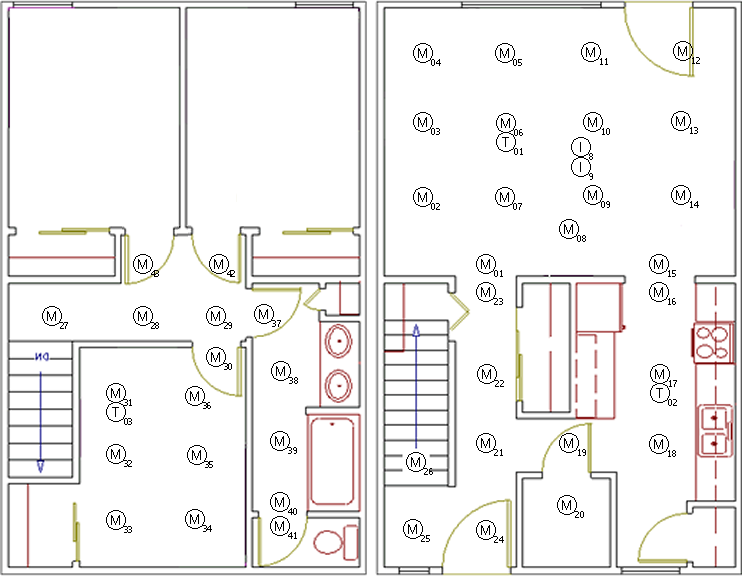
\includegraphics[height=6.3cm]{gfx/Chinook_3_Bedroom_TH}
    \caption{Apartment.\label{fig:house:oner:a}}
  \end{subfigure}%
  \begin{subfigure}[b]{0.3\textwidth}
    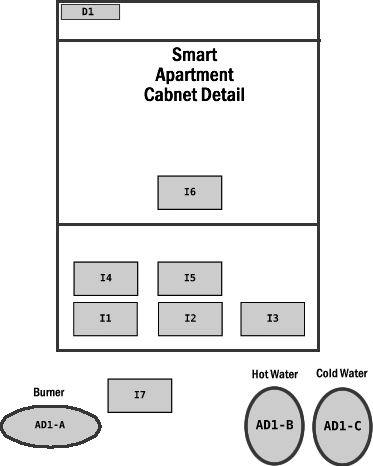
\includegraphics[height=6.3cm]{gfx/Chinook_Cabinet}
    \caption{Kitchen cabined.\label{fig:house:oner:b}}
  \end{subfigure}%
  \caption[The sensor layout of the testbed.]{The sensor layout of the testbed~\citep{cook2009assessing}.\label{fig:house:oner}}
\end{figure}

\noindent The following sensors fitted into the house living space were used:
\begin{description}
\item[M$\Bigcdot\Bigcdot$] motion sensors; boolean signal: \emph{ON}, \emph{OFF};
\item[I$\Bigcdot\Bigcdot$] item sensors: oatmeal, raisin, brown sugar, bowl, measuring spoon, medicine container, phone book; boolean signal: \emph{PRESENT}, \emph{ABSENT};
\item[D01] cabinet door sensor; boolean signal: \emph{OPEN}, \emph{CLOSE};
\item[AD1-A, AD1-B] hot and cold water sensor; numerical, real-valued signal in range 0--1;
\item[AD1-C] burner sensor; numerical, real-valued signal in range 0--1;
\item[asterisk] phone usage; boolean signal: \emph{START}, \emph{END}.
\end{description}

Participants performed five scripted \emph{Activity of Daily Living}:
\begin{description}
\item[Make a phone call] Move to the phone in the dining room; find a specific number in the phone book; dial the number; listen to the message; summarise cooking directions provided over the phone on a notepad.
\item[Wash hands] Move into the kitchen; wash hands in the sink with hand soap; dry hands with a paper towel.
\item[Cook] Cook a pot of oatmeal according to the directions given in the phone message: measure water, pour the water into a pot; boil the water; add oats; put the oatmeal into a bowl; add raisins and brown sugar.
\item[Eat] Take cooked oatmeal; take medicine container; move to the dining room; eat the food.
\item[Clean] Take all of the dishes to the sink in the kitchen; clean them with water and dish soap.
\end{description}

\emph{\#1 WSU Smart Apartment ADL Normal Testbed} dataset has activity structure described above, while \emph{\#2 WSU Smart Apartment ADL Error Testbed} has systematic error introduced:
\begin{description}
\item[Make a phone call] Initially dial the wrong phone number, then redial;
\item[Wash hands] Leave the water on after washing hands;
\item[Cook] Leave the burner on after cooking the oatmeal;
\item[Eat] Forget to take the medicine container to the dining room;
\item[Clean] Clean the dishes without water.
\end{description}

\emph{Listing~\ref{lst:CASASoneR}} shows resulting form these tasks example sensor readings annotated by hand with ground truth.
\begin{figure}[htb]
\lstset{
  captionpos=b,
  frame=single,
  backgroundcolor=\color{Bkgd},
  rulecolor=\color{black},
  language=HTML,
  breaklines=true,
  caption=CASAS single occupier dataset structure.,
  label=lst:CASASoneR,
  float=tb
}
  \begin{lstlisting}
...
2008-02-26 10:52:58.577436 M17   OFF
2008-02-26 10:52:59.648222 M18   OFF       cook       begin
2008-02-26 10:52:59.792264 M17   ON
...
2008-02-26 10:53:43.512642 I02   ABSENT
2008-02-26 10:53:43.978491 I01   ABSENT
...
2008-02-26 10:53:52.112690 AD1-B 0.0421491
2008-02-26 10:53:54.721822 M17   ON        phone_call end
2008-02-26 10:53:55.107910 AD1-B 0.155979
...
  \end{lstlisting}
\end{figure}

      \subsubsection{Multiple residents}
\emph{\#7 WSU Smart Apartment 2009 Two Resident Testbed} is the most popular choice among studies for multiple residents model training and testing. Its testbed design is presented in \emph{Figure~\ref{fig:house:twor}}, with cabinet sensor layout same as in single resident case---shown in \emph{Figure~\ref{fig:house:oner:b}}.\\
\begin{figure}[htb]
  \centering%[width=.45\textwidth] % [height=6.3cm]
  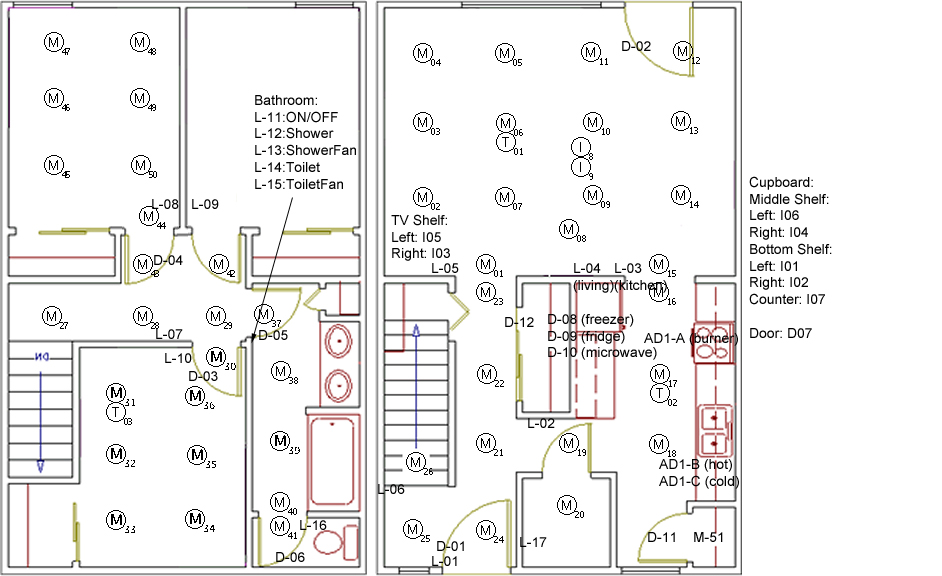
\includegraphics[height=6.3cm]{gfx/sensorlayoutTWOR.jpg}
  \caption[Two residents test-bed sensor layout.]{Two residents test-bed sensor layout~\citep{cook2009assessing}.\label{fig:house:twor}}
\end{figure}

In multiple resident case the sensor set is extended with:
\begin{description}
\item[T$\Bigcdot\Bigcdot\Bigcdot$] temperature sensors; numerical, real-valued signal given in Celsius degrees; and
\item[P$\Bigcdot\Bigcdot\Bigcdot$] electricity usage meter; numerical, integer-valued signal given in kiloWatt Hours.
\end{description}

This dataset was generated with two residents (\textbf{R$\Bigcdot$}): \textbf{R1} and \textbf{R2}, performing their \emph{normal daily activities} (not scripted), therefore, their details are unknown:\\[1em]
\begin{tabular}{ l l l }
  \textbf{R$\Bigcdot$\_Bed\_to\_Toilet}, & \textbf{R$\Bigcdot$\_Personal\_Hygiene}, & \textbf{Wash\_Bathtub}, \\
  \textbf{R$\Bigcdot$\_Work}, & \textbf{R$\Bigcdot$\_Sleep}, & \textbf{Study}, \\
  \textbf{Meal\_Preparation}, & \textbf{Clean}, & \textbf{Watch\_TV}. \\
\end{tabular}
~\\[1em]

Example CASAS multiple occupier dataset is presented in \emph{Listing~\ref{lst:CASAStwoR}}.
\begin{figure}[htb]
\lstset{
  captionpos=b,
  frame=single,
  backgroundcolor=\color{Bkgd},
  rulecolor=\color{black},
  language=HTML,
  breaklines=true,
  caption=CASAS two occupier dataset structure.,
  label=lst:CASAStwoR,
  float=tb
}
  \begin{lstlisting}
...
2009-02-01 02:04:42.039332 P001 2812
2009-02-01 02:05:00.040187 P001 2797
2009-02-01 02:05:26.041714 P001 2784
...
2009-02-01 08:07:57.016506 T004 20.5
2009-02-01 08:07:57.826809 T002 21.5
2009-02-01 08:07:58.442939 T003 22
...
2009-02-06 11:28:36.666599 M09  OFF
2009-02-06 11:28:36.81007  M15  OFF  R2_prepare_lunch  end
2009-02-06 17:16:00.864039 M19  ON   Cleaning          begin
2009-02-06 17:16:01.061019 M21  OFF
...
  \end{lstlisting}
\end{figure}

    \subsection{CASAS issues\label{sec:dataIssues}}
CASAS are the best smart-house datasets that can be used for modelling activity recognition. Unfortunately, they exhibit issues common for every real datasets. Issues such as:
\begin{description}
\item[noise] random sensor activations;
\item[sensor failures] lack of sensor state change notification despite its proper usage; and
\item[incompleteness] signal discontinuity e.g.\ double sensor activation without deactivation in-between
\end{description}
can be identified. All of them cause difficulties in learning activity recognition model.\\

Furthermore, CASAS specific drawbacks hinder their usage. Numeric output of water and burner sensors is unexplained. Additional, for multiple residents datasets not all ground truth activity facts are assigned to people. Also, activities in the latter case are neither scripted nor explained in detail therefore sensor output is tedious to analyse. Without good understanding of human action effects on sensor activations it is relatively hard to design activity recognition model.\\

As ILP activity learning is not documented precise data is required to evaluate its pros and cons. Hence, highly customisable smart-house data generator is required.

  \section{The smart-house generator}
Smart-house data generator created as part of this project is intended to help in activity recognition model design, training and testing. It is highly customisable, hence, it gives user great control over generated data.\\

The user can designing activities of arbitrary structure and complexity and use them to simulate corresponding smart-house output. Then, he can attempt to learn the structure encoded within it. As he knows activity details, he can bypass real data issues (see \emph{Section~\ref{sec:dataIssues}}) and focus on tuning the model. Overcoming one issue at the time greatly benefits model quality and helps to identify its strong and weak points.\\

The tool is open source and published as a \texttt{GitHub} repository together with complete documentation describing design choices, usage details and input-output examples.

    \subsection{Capabilities}
To use the generator, firstly, the user has to describe house by stating room interconnections in form of adjacency matrix.\\

Then, room layout and sensors placement within each room needs to be specified. The room dimensions are required together with list of wanted sensors. The design is based on Cartesian coordinates with origin in bottom left corner of the room.\\
For motion sensors: ID, position and range has to be specified. Sensors of these type detect motion radially from their location.\\
Item sensors are defined with: ID, position, and its human readable name.\\
Finally, door location is needed for layout completeness. They are encoded with \texttt{door} keyword, their coordinates and name of a room they lead to.\\
Example definition of each sensor type (order preserved) is given in \emph{Listing~\ref{lst:sensorLayout}}.\\

\begin{figure}[htb]
\lstset{
  captionpos=b,
  frame=single,
  backgroundcolor=\color{Bkgd},
  rulecolor=\color{black},
  language=HTML,
  breaklines=true,
  caption=Example sensor definitions.,
  label=lst:sensorLayout,
  float=tb
}
  \begin{lstlisting}
m13  4.5 1   1
i78  5.5 0.5 phone_book
door 0   0.5 hall
  \end{lstlisting}
\end{figure}

Subsequently, item sensors characteristics have to be specified. Each item, like TV, takes some time to use---average TV watching time. It is simulated by drawing a sample of Gaussian distribution with user specified mean and standard deviation. This feature is mainly used for simple activities but the time can be altered in activity specification script (see next paragraph).\\
Walking is simulated in the same way---single step size and time together with their standard deviations have to be specified.\\

Finally, activity script used to simulate interaction with sensors has to be provided. Arbitrary number of activities (they can be nested) for multiple people can be defined. Each script is specified with start position and any of the following atomic actions can be issued: go to room, go to location within the room, use item (simulate previously defined time), pick up any item or start any device, put down the item or turn off the device. For more complex activities any command can be used between starting/taking and stopping/returning any device/item.\\
Curly brackets together with activity name are used to surround atomic actions contributing towards this activity. Example script is given in \emph{Listing~\ref{lst:path}}.\\

\begin{figure}[htb]
\lstset{
  captionpos=b,
  frame=single,
  backgroundcolor=\color{Bkgd},
  rulecolor=\color{black},
  language=HTML,
  breaklines=true,
  caption=Example activity script.,
  label=lst:path,
  float=tb
}
  \begin{lstlisting}
>ResidentA>
origin(hall)
go(kitchen)

cook{
  start(cabinet)
    do(oatmeal)
    do(pot)
  stop(cabinet)

  do(water_cold)

  start(burner)

  watchTV{
    go(living_room)
    do(tv)
  }watchTV

  go(kitchen)
  stop(burner)
}cook
<ResidentA<
  \end{lstlisting}
\end{figure}

Presented here tool is capable of generating arbitrarily complex user defined activities by specifying their atomic actions. The generator can simulate multiple residents interacting with the house simultaneously.\\
Additionally to CASAS-like signal output, precise ground truth is recorded.\\

Datasets generated for ILP activity recognition models are using house design presented in \emph{Figure~\ref{fig:simHouse}} with systematic grid of motion sensors fitted within each room.

\begin{figure}[htb]
  \centering% [width=.9\textwidth]
  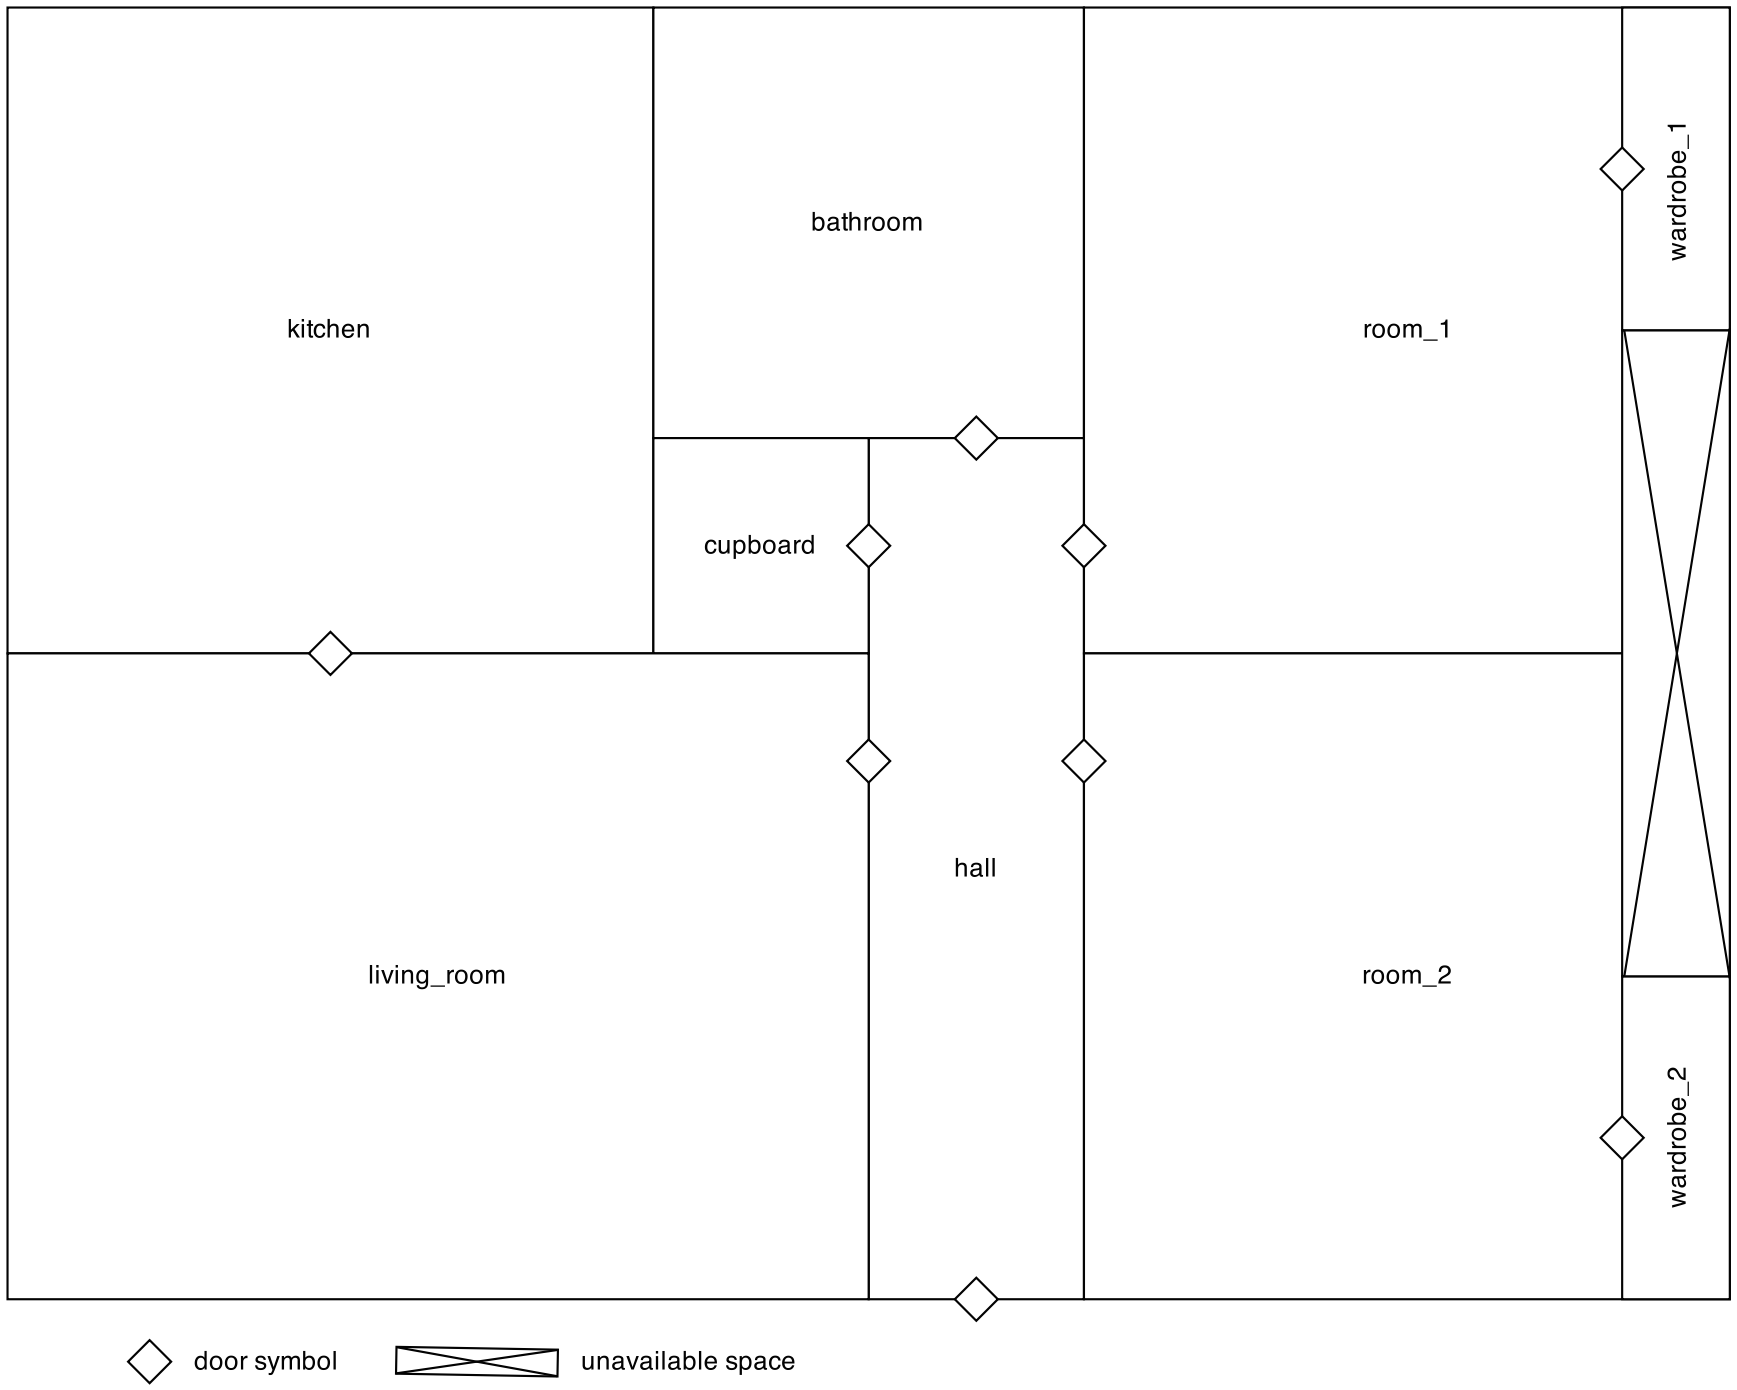
\includegraphics[height=7.3cm]{./gfx/room_layout}
  \caption{Simulated house room layout.\label{fig:simHouse}}
\end{figure}

    \subsection{Advantages}
Created smart-house data generator is flexible and highly customisable. The simulated resident can perform tasks of arbitrary complexity ranging from simple motion to nested activities each using different combination of available items. Moreover, the output signal can be distorted with various kinds of noise and randomness.\\

The main advantage of proposed here simulation technique is detailed knowledge of ground truth, which is based on input activity script. Availability of various kind of simulation statistics can be used to visualise sensor behaviour and debug activity model trained on generated data.\\

Finally, the raw signal output of the generator is given in widely accepted CASAS format. Therefore, simulations made with described here tool can be used with all activity recognition systems based on CASAS datasets.

    \subsection{ILP ready}
The smart-house data generator was designed with ILP model construction in mind, therefore, it outputs \texttt{Prolog} facts needed for this purpose. Information such as house specific background knowledge and positive \& negative examples required by ILP algorithm is recorded.\\
Additionally, detailed sensor activations, time-location and activity structure informations are available for manual analysis of output signal.

    \subsection{Proof of concept}
The value of presented here smart-house data generator can increase significantly if it can be proven to produce real-like datasets. Proof for single resident case is sufficient as multiple residents house is based on combination of multiple single agent simulations. The latter effect is achieved by special handling (preserving sensor states) of cases when agents cross each other's paths and interact with common device or item.\\
Presented here proof is based on \emph{similarity comparison} of ILP models learnt on CASAS and generated datasets.\\

The evaluation is based on...\\
>EVALUATION RESULTS<

  \section{Knowledge representation of spatio-temporal data}
Activity learning method described here requires signals represented as logical facts. ILP system used in this study is written in \texttt{Prolog} programming language therefore, all data has to be expressed in thereof predicates. This requirement causes some problems introduced by sensor type variety.\\

The most common sensor output are binary variables: on-off, present-absent, opened-closed, etc.\ produced by motion and item sensors. Expressing them in predicates is straight-forward as their search space is finite---a set containing two elements.

    \subsection{Unbounded sensor readings}
Another type of sensor output are real and whole numbers. Handling these quantities is well known and broadly documented issue in Artificial Intelligence and Logic Programming. As \texttt{Prolog} is a language based on search space traversal numbers i.e.\ unbounded variables have infinite (unbounded) search space.\\

When sensor output is numerical it is converted to Boolean space by simple shareholding. The critical value is hand-picked based on observation of output values.\\
A special case of unbounded readings is time.

    \subsection{Time representation\label{sec:timeRepresentation}}
Date-time is complex object encoding many useful information. Unfortunately, its human readable format---YYYY-MM-DD HH:mm:SS.ssssss---is of no use in computer science. Converted to machine language it is expressed as a \emph{timestamp}---number of seconds elapsed since epoch dated on 00:00:00, 1\ts{st} January 1970, UTC.\\

For my study I chose to represent time in 4 different way:
\begin{description}
\item[absolute] is timestamp represented in micro-seconds ($\mu$-seconds: $10^{16}s$) rather than seconds,
\item[relative] is number of micro-seconds elapsed since first sensor activation in the dataset,
\item[sequenced] is a sequential number of sensor activation in the dataset starting with $0$,
\item[windowed] is sequential number of fixed-time-interval window that the event fall into; the first time-windows starts on first sensor activation and has ID $0$; window of 5 seconds is used in the study.
\end{description}
Representation examples are shown in \emph{Figure~\ref{lst:timerepresentation}}.\\

\begin{figure}[htb] % [breaklines]
  \begin{minted}[bgcolor=Bkgd,frame=leftline]{Prolog}
sensor(m12, true, relative, 4007842 ).
sensor(m12, true, absolute, 1430004781866056 ).
sensor(m12, true, sequence, 2 ).
sensor(m12, true, windowed, 0 ).

sensor(m13, false, relative, 5994214 ).
sensor(m13, false, absolute, 1430004783852428 ).
sensor(m13, false, sequence, 3 ).
sensor(m13, false, windowed, 1 ).
  \end{minted}
  \caption{Signal represented as \texttt{Prolog} facts.\label{lst:timerepresentation}}
\end{figure}

As no single time representation is best for ILP application all four were tested and evaluated. \emph{Sequence} is most suitable in search space environment---the numbers are not sparse therefore the application can easily iterate through them without large computational overhead.\\
For this reason I chose this representation as the main time format. Despite being helpful in ILP scenario sequential number is highly uninformative. It lacks basic information such as time of day or possibility to be transformed into time elapsed since last sensor reading.\\

To enrich source of information used by learning algorithm \emph{timestamp} representation is used. Following directly from sequence number it can be easily accessed. With such detailed representation of micro-second accuracy, precise time elapsed since any event can be calculated.\\
Moreover this value can be thresholded hence discretised to produce bounded variables such as:
\begin{description}
\item[time of year] winter, summer, autumn, spring;
\item[month] January, February, March, etc.;
\item[time of day] morning, afternoon, evening, night;
\end{description}
and similar. In particular, in ILP and AI such values a lot easier to work with than numbers.\\

The remaining two representations: \emph{relative} and \emph{windowed} are of little use in presented here learning approach.

    \subsection{Background knowledge\label{sec:data:bkg}}
Background knowledge is a general name for a place containing all the information relevant to model learning. By far, it is the most important component of ILP containing building blocks of target model. Moreover, it is a place for logical representation of signals and all relevant rules interacting with them. Additionally, it contains any information not contained or implicit in the raw signals.\\

From large enough sample of smart-house data it is feasible to infer room layout and interconnections, unfortunately this task is computationally complex and impractical in most cases. ILP comes with help in such scenarios as it is ready to use any information not given in raw signals by reading it from background knowledge. Room connections information is great feature as it helps to predict motion trajectory and person's location.\\
Sensor allocation---placement in rooms---is another information not given in raw signal. With help of sensors location, sensor activations can be translated into room name in which the activity is happening.\\
Examples of information used in the background knowledge file is given in \emph{Figure~\ref{lst:bg}}. Fact \texttt{connected\_\_} informs about room connections via doors; \texttt{sensorInRoom} contains information where sensor of given ID is placed; \texttt{sensorActivity} is used with all item and appliance sensors and assigns human readable name to sensor ID; finally, \texttt{sensorInField} tells in range of which motion sensor item or appliance is located.\\

\begin{figure}[htb] % [breaklines]
  \begin{minted}[bgcolor=Bkgd,frame=leftline]{Prolog}
connected__(   bathroom, hall    ).

sensorInRoom(  m61     , bathroom).

sensorActivity(ad1-c   , burner  ).

sensorInField( ad1-b   , m83     ).

aPriori(tv    , watchTV   ).
aPriori(burner, cook      ).
aPriori(phone , phone_call).

bedroom(residentA, bedroom1).
bedroom(residentB, bedroom2).
  \end{minted}
  \caption{Background knowledge facts snippet.\label{lst:bg}}
\end{figure}

Apart from house layout information \emph{prior believes} of any kind can be used in background knowledge---see \texttt{aPriori} keyword \emph{Figure~\ref{lst:bg}}. A priori information such as likely place of activity, device or item required to complete it, and the order of activities are of invaluable help. For example, watching TV is most often associated with living room and a meal cannot be eaten unless it has been cooked. It is a fact that watching television requires TV to be on, cooking is happening on a hob and to make a phone call one needs to use a phone.\\
With multiple residents in a house information such as bedroom assignment helps to distinguish them (\texttt{bedroom} keyword in \emph{Figure~\ref{lst:bg}}).\\

\begin{figure}[htb] % [breaklines]
  \begin{minted}[bgcolor=Bkgd,frame=leftline]{Prolog}
location(Time, Location) :-
  (sensorInRoom(SensorID, Location),
   sensor_state(SensorID, true, Time),
   Time >= 0, !  )
  ;( !, Time > 0,
    location(Time-1, Location) ).
  \end{minted}
  \caption{Example rule.\label{lst:bg:rule}}
\end{figure}

Another component of background knowledge are \texttt{Prolog} rules interacting with facts and signals---they can be understood as \emph{feature extractors}. Rule example is shown in \emph{Figure~\ref{lst:bg:rule}}; it queries \emph{where} (room name) a person is at given \emph{time}.\\

Background knowledge can be also understood as \emph{proxy} between raw signals and high level activity rules. As output rules are based on room, item, appliance names and not sensor IDs they are universal. Already existing model can be applied to any other house by using specific to that place background knowledge.\\
Finally, learnt rules can be used in future iterations of learning process by appending them to the background knowledge.


    \subsection{Positives and negatives\label{sec:data:posneg}}
The final component of ILP are positive and negative examples of model to learn. Sample facts for both single and multiple occupiers are presented respectively in \emph{Figure~\ref{lst:singleposneg}}~\&~\emph{\ref{lst:multiposneg}}.\\

\begin{figure}[htb] % [breaklines]
  \begin{minted}[bgcolor=Bkgd,frame=leftline]{Prolog}
activity(cook  , 47).
activity(eat   , 51).
activity(eat   , 52).
activity(eat   , 53).
activity(washUp, 59).
activity(washUp, 60).
  \end{minted}
  \caption{Positives and negatives for single resident.\label{lst:singleposneg}}
\end{figure}

These examples use \emph{sequence} representation of time to express when (and by whom) activity \emph{is}: positives, and \emph{is not}: negatives done. Both types have common structure and are separated into two different files to be distinguishable.\\

\begin{figure}[htb] % [breaklines]
  \begin{minted}[bgcolor=Bkgd,frame=leftline]{Prolog}
activity(sleep, 14, residentA).
activity(sleep, 15, residentA).
activity(sleep, 16, residentA).
activity(sleep, 17, residentA).
activity(useBathroom, 4, residentB).
activity(useBathroom, 5, residentB).
activity(useBathroom, 6, residentB).
activity(useBathroom, 7, residentB).
  \end{minted}
  \caption{Positives and negatives for multiple resident.\label{lst:multiposneg}}
\end{figure}

For each activity the sets of positive and negative examples have to be disjoint with regard to time. The ILP system generalises positive examples into complex rules containing in body references to sensor states under restriction of not covering any or some negative examples.

  \section{The converter}
The next step in model learning is data conversion from CASAS-like log format to \texttt{Prolog} \emph{knowledge representation} i.e.\ state signal readings as logical facts. The converter is capable of handling both single and multiple residents datasets. To this end, number of conversion steps is need.\\

Real-valued signals like AD1-B water sensor (see \emph{Listing~\ref{lst:CASASoneR}}) are threshold and discretised. Binary sensor output is unified to values \emph{true} and \emph{false}. The time-date information is converted into four described in \emph{Section~\ref{sec:timeRepresentation}} representation.\\
Moreover, the converter uses activity and person ID information given in 4\ts{th} and 5\ts{th} column of the data to generate positive and negative examples needed for learning activity model with \texttt{Aleph}.

  \section{The cross-validation}
Once the data is converted and passed to \texttt{Aleph} the model in form of rules describing activities is produced. To evaluate their quality 10-fold cross-validation is performed.\\
For each script of activities 10 data recordings are gathered together with corresponding model learnt with ILP. Then, each sample model is evaluated on the remaining nine datasets and the results are checked against corresponding ground truth. After testing all possible model-data combinations overall and per-label accuracy and is reported. The output of cross-validation framework is on of the diagnostics used to evaluate model performance.


%===============================================================================
%===============================================================================
%===============================================================================
%===============================================================================
%===============================================================================
\chapter{Inductive Logic Programming\label{ch:ILP}}
\citet{plotkin1972automatic} in early 1970s and \citet{shapiro1983algorithmic} in early 1980s created foundation of \emph{Inductive Logic Programming} (ILP). Both authors introduced techniques and tools to learn \emph{first-order formulas} (parametrised rules that are the core of the ILP) describing chosen object based on a set of facts. Since then, ILP techniques found number of interdisciplinary applications with new tools being created now and then for rules learning purposes.

  \section{Inductive Logic Programming}
The concept of Inductive Logic Programming is based on fusion of two well known techniques: \emph{inductive learning} and \emph{logic programming}. The first component facilitates building model from available observations and generating new knowledge form experience. The latter, introduces a powerful representation of knowledge as \emph{first-order logical rules}~\citep{muggleton1994inductive,muggleton1995inverse}.

    \subsection{Logic programming}
\emph{Propositional logic} widely used in machine learning models is ``\emph{weaker}'' than first-order logic used in ILP. A propositional sentences (rules) are made of facts combined with \emph{logical connectives} such as: not ($\neg$), and ($\land$), or ($\lor$), existence ($\exists$), etc.. Such sentence can only be evaluated to true or false based on predicates in its body e.g.\
$$\left(\left(\texttt{sensorM42} \land \texttt{sensorM47}\right) \lor \left(\texttt{sensorM27} \land \texttt{sensorM30}\right)\right) \land time = 40$$
where \texttt{sensor$\Bigcdot\Bigcdot\Bigcdot$} denotes sensor $\Bigcdot\Bigcdot\Bigcdot$ being on, is true if either both \texttt{sensorM42} and \texttt{sensorM47} or \texttt{sensorM27} and \texttt{sensorM30} are simultaneously on at time $40$.\\

Thanks to first-order logic ILP overcomes mentioned above ``limited representation formalism'' (expressing data in form of a propositional logic). Many problems considered hard to solve while expressed propositionally can be easily tackled with ILP. The power of first-order logic lies in expressing its sentences with \emph{parametrised} predicates. Use of domain specific quantified variables alters logical state of sentence based on their input and output therefore facilitates expressing complex relations. An example of first-order activity rule: \texttt{activity(A,B)} where variable \texttt{A} denotes activity ID and \texttt{B} time, is given below. The rule illustrates the dependence between predicates via free variables.\\
\begin{eqnarray*}
&\texttt{activityOrder(B,A)} \land \texttt{location(B,livingRoom)} \land \\
&\texttt{outOfCabinet(B,C)} \land \texttt{medicineInList(C)}
\end{eqnarray*}
The major limitation of first-order logic is its restriction to finite variable domains---it cannot describe rules built on infinite sets like real or natural numbers.\\

Finally, ILP does not have difficulties in incorporating substantial background knowledge in form of first-order sentences to the model. This feature is not very common among machine learning models, nevertheless, use of domain knowledge is ``essential for intelligent behaviour''~\citep{muggleton1994inductive}.

    \subsection{Inductive learning}
The second component of ILP is inductive learning: constructing \emph{first-order clausal theories}. Such hypotheses are based on combining background knowledge with facts representation of positive and negative examples; see \emph{Figure~\ref{fig:ilp}}.\\
\begin{figure}[htb]
  \centering
  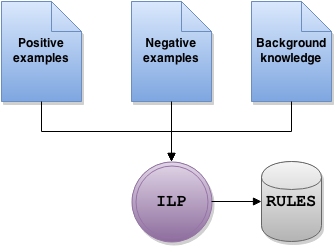
\includegraphics[scale=.5]{./gfx/ilp}
  \caption{ILP scheme\label{fig:ilp}}
\end{figure}
ILP aims at building theory that under consideration of background knowledge explains facts: covers as much positive examples as possible without covering and or most of negative examples. To this end, it uses \emph{induction} as a basic mode of inference: generalization of specific observations to theories, rather than deduction: transforming general theories to the more specific clauses.

    \subsection{Applications}
The rules produced with ILP are human readable unlike models produced by majority of machine learning solutions, what gives it great advantage over competition. Easy to understand rules means that the logic models are arguably easy to manipulate. They can be changed by simply adding, deleting, and modifying clauses or literals.\\
Such model representation is invaluable in \emph{scientific theory formation} and problems where data cannot be easily represented in attribute-vale language. ILP is widely used in structure-activity prediction for drug design~\citep{king1992drug,michael1992modelling} and protein secondary-structure prediction~\citep{muggleton1992protein}. It is also popular tool in computer science as: programming assistance, algorithmic debugging, program testing and verification, and reverse engineering~\citep{shapiro1983algorithmic,bergadno1993inductive,bratko1993inductive}.\\

The two most popular \texttt{Prolog} ILP implementations are \texttt{Aleph}\footnote{\url{http://www.cs.ox.ac.uk/activities/machlearn/Aleph/aleph.html}} and \texttt{Progol}\footnote{\url{http://www.doc.ic.ac.uk/~shm/progol.html}}. \texttt{Aleph} is chosen for this study due to its comprehensive documentation availability and ease of use on contemporary platforms.

  \section{\texttt{Aleph}}
\texttt{Aleph}: A Learning Engine for Proposing Hypotheses, is \texttt{Prolog} based Inductive Logic Programming system developed at Oxford University by \citeauthor{muggleton1994inductive}. It is compatible with two most popular \texttt{Prolog} language implementations: \texttt{YAP}---Yet Another Prolog, and \texttt{SWI-Prolog}.

    \subsection{Input files}
\texttt{Aleph} infers hypotheses using three files, the first two contain positive and negative examples of target rule model, the third encodes program settings and additional informations.

      \subsubsection{Background}
Background file contains \texttt{Aleph} configuration and target model specification; see example given in \emph{Figure~\ref{lst:alephSettings}}. Settings such as used evaluation function, allowed maximal number of negative examples covered by a single target rule, and minimal number of positive examples that each rule has to cover are used.\\
Additionally, user provides target rule specification. Based on presented example the target \texttt{activity} rule has $2$ variables (is of \emph{arity} $2$): (constant, \#) activity ID and (input, +) integer representing time. The body of the rule can contain arbitrary number of \texttt{device} and \texttt{location} predicates each having $2$ variables. The first takes integer time input and constant device ID; the latter integer time input and constant room ID.\\
Finally, target model constrains can be specified (\texttt{false} keyword): in presented example no two activities can happen at the same time.\\
\begin{figure}[htb] % [breaklines]
  \begin{minted}[bgcolor=Bkgd,frame=leftline]{Prolog}
% Internal settings
:- set(evalfn, wracc).
:- set(noise , 3    ).
:- set(minpos, 1    ).
% Determinations
:- determination(activity/2, device/2  ).
:- determination(activity/2, location/2).
% Mode declarations: rule head definition
:- modeh(*, activity(#activityIDs, +integer) ).
% Rule body definition
:- modeb(*, device(+integer, #deviceIDs)).
:- modeb(*, location(+integer, #roomIDs)).
% Constrains
false :-
  activity(Activity1, T),
  activity(Activity2, T),
  not(Activity1 = Activity2).
  \end{minted}
  \caption{Example \texttt{Aleph} settings.\label{lst:alephSettings}}
\end{figure}
Therefore, target rules are of the form \texttt{activity(ActivityID, Time) :- $\Bigcdot$}.\\

Additionally to presented above \texttt{Aleph} settings, background knowledge file also contains facts and rules discussed is \emph{Section~\ref{sec:data:bkg}}.

      \subsubsection{Positives}
Positive examples file lists activity facts of the form \texttt{activity(ActivityID, Time).} to indicate at which time points the activity was happening in a data. Example file is discussed in \emph{Section~\ref{sec:data:posneg}}.

      \subsubsection{Negatives}
Negative examples file is of the same form as positive example file. It indicates time-points when activities were not undertaken. In presented here learning scenario the negative time-points are set complement of positives examples and are bounded from below by $0$ and from above by number of sensor readings in the data set; see \emph{Figure~\ref{fig:timepoints}} for reference. Example file is discussed in \emph{Section~\ref{sec:data:posneg}}.
\begin{figure}[htb]
  \centering
  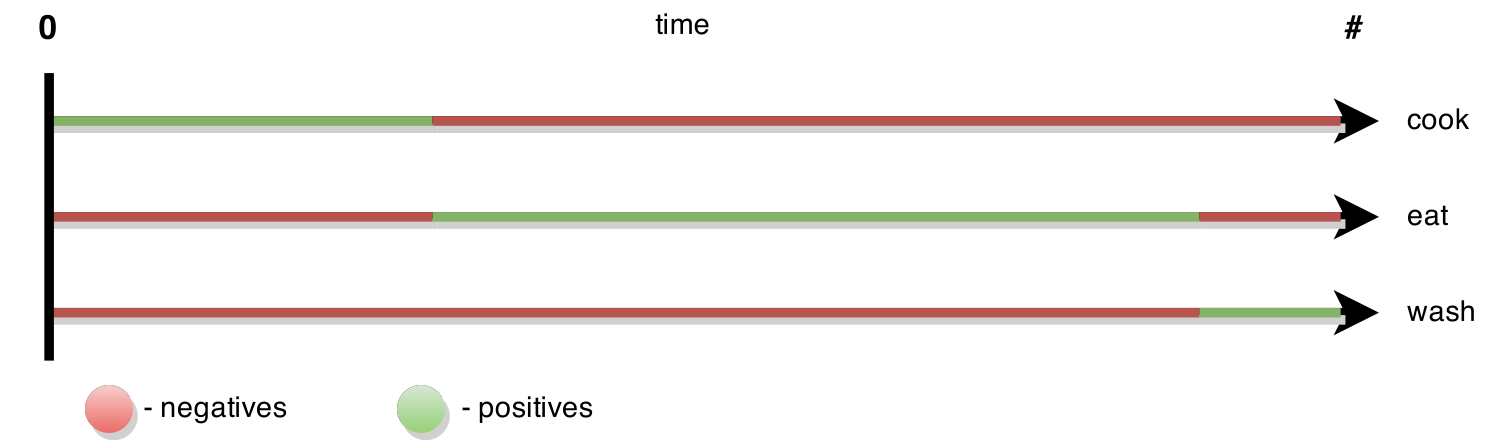
\includegraphics[width=.85\textwidth]{./gfx/activityStructure}
  \caption{Activity structure example.\label{fig:timepoints}}
\end{figure}

    \subsection{\texttt{Aleph} output}
Based on input data \texttt{Aleph} outputs set of rules compliant with given specification. Presented in \emph{Figure~\ref{lst:alephSettings}} settings could result in first from the top rule given in \emph{Figure~\ref{lst:alephOut}}. It does not contain free variables in the body hence can be expressed in propositional logic.\\
The second one is more complex yet still propositional. \texttt{outOfCabinet(A,[none])} predicate gives list of items taken out of cupboard at time \texttt{A}.\\
The third activity rule is a \emph{singularity}. Positive example \texttt{activity(clean,87).} is outputted as the ILP algorithm could not generalised it to proper rule without breaking any of the restrictions imposed by the background file. Such rules are pruned out prior to cross-validation.\\
\begin{figure}[htb] % [breaklines]
  \begin{minted}[bgcolor=Bkgd,frame=leftline]{Prolog}
activity(wash_hands,A) :-
  device(A,water_hot).

activity(wash_hands,A) :-
  outOfCabinet(A,[none]),
  waterUsed(A).

activity(clean,87).
  \end{minted}
  \caption{Example activity model.\label{lst:alephOut}}
\end{figure}

An example of more advanced, first-order logical rule is presented in \emph{Figure~\ref{lst:bg:rule}}. Free variables present in the rule body ensure clauses interaction.

    \subsection{The basic algorithm}
Generally speaking, inductive logic programming is a \emph{search problem}. The algorithm traverses through \emph{candidate solution space} i.e.\ set of ``well-formed'' hypotheses, to find the most suitable one. ILP problem can be solved using na\"{\i}ve generate and test algorithm however, this approach is highly inefficient. The most suitable solution has four steps: select example, build most-specific-clause, search, and remove redundancies~\citep{muggleton1994inductive}.

      \subsubsection{Select example}
Select positive example that is not yet covered by learnt rule form the positives set. If all were tested stop the procedure.

      \subsubsection{Build most-specific-clause}
Also known as \emph{saturation step}. Construct \emph{bottom clause}: definite clause with many literals that is most specific given that it entails previously selected example and complies with provided restrictions.

      \subsubsection{Search}
Also known as \emph{reduction step}. Search through subsets of previously found literals to build more general clause that complies with given restriction.\\
More general clause can improved performance by covering more than one positive example.

      \subsubsection{Remove redundancies}
Also known as \emph{cover removal}. Memorise the clause with the best score (coverage) and remove positive examples made redundant (covered) by new clause. Return to \emph{Select example} step.

  \section{Applications to spatio-temporal data}
With a bit of tuning ILP can be applied to spatio-temporal data with quite good results. Despite difficulty in handling numerical values rule based model is highly suitable for activity recognition task.\\

Arbitrary information that can be appended to background knowledge greatly improves raw signal handling. \texttt{Prolog's} \emph{negation as failure} is consistent with lacking sensor state. \texttt{Prolog} assumes that any sensor is off if it cannot be ``proven'' to be on; regardless of whether it does not exist at all or it has not been activated yet, hence, according to data it is neither on nor off. This approach helps in smoothing out sensor readings e.g.\ if current location cannot be inferred from available sensor readings the model assumes last known location.\\

Moreover, output model written in \texttt{Prolog} is human readable therefore relations in data revealed by ILP can be understood and used to improve the model. The output theory can be also easily modified and enclosed within meta-rules. This practice is an easy fix for prediction continuity issue.\\

Finally, expressing hierarchy in rule based model can be easily achieved by placing one rule in the body of the other or conditioning only on some subset of body literals. The concepts of rule generalisation and specialisation directly correspond to moving up and down the hierarchical structure.

  \section{Closed Concept \& Least General Generalisation}
A \emph{closed concept} is a concept that includes all implicitly understood conditions. For example rule:\\
\begin{minted}[bgcolor=Bkgd,frame=leftline]{Prolog}
activity(wash_hands,A) :-
  device(A,water_hot),
  location(A,kitchen).
\end{minted}
and:\\
\begin{minted}[bgcolor=Bkgd,frame=leftline]{Prolog}
activity(wash_hands,A) :-
  device(A,water_hot).
\end{minted}
both have the same coverage of positive examples, but the first is more general, therefore, it is a closed concept. In other words, it is the \emph{least general generalisation} (LGG) of chosen positive example.\\

Due to \texttt{Aleph} search step, bottom clause i.e.\ LGG of currently selected positive example, is pruned of redundant (from performance perspective) literals, hence, activity details are lost. In the example given above location of washing hands is reduced. These disregarded informations are of great importance for feature construction and data narrative (see \emph{Section~\ref{sec:narrative}}).\\

It is possible to generate closed concept of activity rules in \texttt{Aleph} by disabling search step. To achieve this, search setting has to be overwritten: \texttt{:- set(search, false).}.

  \section{Feature discovery and feature extraction}
Building a data model with ILP requires right features to be available in background knowledge. By large, ILP algorithm searches through feature space to find their most suitable combination for each activity model. In presented here scenario features are understood as rules interacting with both, raw signals and each other in order to extract knowledge relevant to model.\\
Designing such rules can be understood as feature construction and requires awareness of ``activity script'' used to generate the data regardless of their origin: simulation or human actor interacting with smart-house. ``Activity script'' can be both: general description of activities or ordered list of tasks to be perform by an agent.\\

Rule body of output activity model can be then examined to analyse relations between features and activities. Interesting predicates can be then applied directly to raw dataset to generate new feature vectors. It is widely known that well crafted features can boost performance of any machine learning model. Additionally, more informative LGG of output rules can be checked.\\
Features used for both single and multiple resident models are discussed in detail in \emph{Section~\ref{sec:single:features}~\&~\ref{sec:multiple:features}}.


%===============================================================================
%===============================================================================
%===============================================================================
%===============================================================================
%===============================================================================
\chapter{Sequential multi-class model\\(single resident)\label{ch:smcm}}
% presented above example both \texttt{location} and \texttt{device} rules can be transformed to become features. Rebuilt dataset may become more ``informative'' than the original one, therefore, it can improve classification carried out with variety of different machine learning models.
  \section{Evaluation measures}
  \section{Simple synthetic dataset}
% Bias is introduced on location.
% Example of ILP rules learnt with \texttt{Prolog} are shown in \emph{Listing~\ref{lst:eg}}.
  \section{CASAS \#2}
    \subsection{Synthetic CASAS \#2}
% narrated datasets
    \subsection{Genuine CASAS \#2}
% narrated datasets
  \section{Discontinuity}
% Continuity rule --- introducing bias\\
% Meta-rule -- smoothing out predictions
  \section{Model generality}
% Generality of learnt rules (synthetic <--> genuine) Results overview
  \section{Overlapping activities}
% single resident multi-label case
  \section{Features\label{sec:single:features}}


% \vspace{1em}
% \begin{figure}[htb]
% \lstset{
%   captionpos=b,
%   frame=single,
%   language=Prolog,
%   breaklines=true,
%   caption=Example of target rules.,
%   label=lst:eg,
%   float=tb
% }
% \begin{lstlisting} % [breaklines]
%   \begin{minted}[bgcolor=Bkgd,frame=leftline]{Prolog}
% activity(Person, cooking) :-
%   location(Person, TimeWindow, kitchen), device(TimeWindow, hob).
% activity(Person, watchingTV) :-
%   location(Person, TimeWindow, livingRoom), device(TimeWindow, tv).

% location(Person, TimeWindow, kitchen) :-
%   sensor(1, on, TimeWindow), sensor(5, on, TimeWindow).
% location(Person, TimeWindow, livingRoom) :-
%   sensor(2, on, TimeWindow), sensor(7, on, TimeWindow).

% device(TimeWindow, hob) :-
%   sensor(101, on, TimeWindow).
% device(TimeWindow, tv) :-
%   sensor(105, on, TimeWindow).
%   \end{minted}
%   \caption{Caption.\label{lst:label}}
% \end{lstlisting}
% \end{figure}


%===============================================================================
%===============================================================================
%===============================================================================
%===============================================================================
%===============================================================================
\chapter{Multi-label model\\(multiple residents)\label{ch:mlm}}
  \section{Evaluation measures}
  \section{Bathroom excursion}
    \subsection{Movement case}
    \subsection{Still case}
  \section{CASAS \#9}
  \section{Features\label{sec:multiple:features}}


%===============================================================================
%===============================================================================
%===============================================================================
%===============================================================================
%===============================================================================
\chapter{Summary\label{ch:summary}}
My work in the field of activity recognition focused on identifying capabilities and limitation of inductive logic programming technique in learning activities of daily living recognition model from smart-house data. To this end, I recognised issues with real dataset causing learning difficulties. To mitigate these issues and examine ILP capabilities I built highly customisable smart-house data generator. It allowed me to focus on building activity recognition model for single and multiple residents on synthetic data, therefore, not worry about technical signal issues like noise, incompleteness, and lack of detailed ground truth. Finally, after identifying ILP capabilities I addressed handling real data issues.

  \section{Smart-house data generator}
Data generator as a helpful tool for building and testing models.\\
Close enough within reasonalbel degree. ILP can be used as one of models for activity recognition: its strong points not available (or hard to achieve) in other models.\\

  \section{Rule based Activity Recognition Model}
Onlybacisc activitry recognition probelm are addressed identifired in literature and common in data.

  \section{Work evaluation}
what my results mean to general public.\\
Undenstendable rules -> undenstand data and not just use black-box methods which have good results.\\
Design features on known datasets -> they usualy are repetitive -> therefore structure in unscripted data can be identified.

  \section{Further development}
Presented here strong points of rule based models can be utilised by including it in an activity recognition classifier ensemble. By combining it with other techniques best features of each classifier can be used and majority of individual weaknesses mitigated. Therefore, behaviour of ILP model should be evaluated in ensemble environment to identify potential performance improvements.

    \subsection{Model complexity}
Rule models presented in this paper are restricted to basic activities of daily living recognition for single and multiple residents. As the complexity of datasets can be arbitrarily increased by introducing new activities further learning attempts can be done. Moreover, data noise and incompleteness influence on ILP learning capabilities can be systematically evaluated. Finally, influence of common to people, systematically introduced errors while performing set activities can be examined for ILP framework.

    \subsection{Data Narrative concept\label{sec:narrative}}
Most commonly used visualisation techniques nowadays are tables, graphs, and diagrams. Unfortunately, such charts often need expertise in a field to be correctly interpreted. Moreover, aforementioned methods often trade-off clarity for completeness of shown data hence make it difficult for a broad audience to see the big picture.\\

\emph{Narrative Analysis} describes data with natural language: a \emph{succinct plain English description} of events encoded in selected time-space window. Despite its power, this form of data representation has been under-appreciated and devoted little attention in recent years.\\
Data narration can be found in modern smart-phone weather and calendar applications where instead of detailed weather forecast or hour-by-hour calendar schedule, one sentence description is presented to the user. In combination with other visualisation techniques it has been proven as an effective method of expressing corporate financial data. Moreover, deep learning algorithms have been applied to images to generate captions---succinct scene descriptions~\citep{vinyals2014show}.\\

Successful adaptation of \emph{narrative analytics} to smart-house data would greatly benefit healthcare applications. Delivering comprehensible activity description within given time-space window and with level of detail tuned to a particular recipient would provide invaluable monitoring and diagnostic tool for day-care personnel and medical staff. Activities transparently expressed as English sentences gives possibility to quickly understand status of the system without time-consuming raw-data or charts interpretation.\\
Furthermore, proposed here descriptive mechanisms could be extended to become a query-enabled database. In such a model user could ``ask'' a question in natural language to get narrative answer instead of numerical vector.\\

% generative framework
Proposed in this paper rule based activity recognition model can become foundation for advanced \emph{Narrative Analtics} tool. \texttt{Prolog} is well known for great natural language processing capabilities, therefore, activity rules can be translated into plain English data description.

\begin{center}
\noindent \line(1,0){250}
\end{center}

\bibliography{yhpargoil}{}
\bibliographystyle{plainnat}
% \bibliographystyle{plain}

\end{document}

% useful expressions:
%% aggregate signal
% \citeauthor{BiBTeX_reference}
%  as opposed to
